\documentclass[11pt, a4paper, twoside]{article}

\usepackage[margin=2cm]{geometry}
\usepackage{graphicx}
\usepackage{booktabs}
\usepackage{tabularx}
\usepackage{longtable}
\usepackage{multirow}
\usepackage{amsmath, amssymb}
\usepackage{siunitx}
\usepackage{enumitem}
\usepackage{titlesec}
\usepackage{fancyhdr}
\usepackage[hidelinks, bookmarks=true, bookmarksdepth=3]{hyperref}
\usepackage{xcolor}
\usepackage{parskip}
\usepackage{pgfplots}
\usepackage{tikz}
\usepackage{bytefield}
\usepackage{listings}
\usepackage{tocloft}
\usepackage{pdfpages}

\pgfplotsset{compat=1.18}
\usetikzlibrary{arrows.meta, positioning, calc, shapes.geometric, patterns, decorations.pathreplacing}

% ── Colours ───────────────────────────────────────────
\definecolor{accentblue}{HTML}{4A9EFF}
\definecolor{accentred}{HTML}{FF5555}
\definecolor{accentgreen}{HTML}{50C878}
\definecolor{accentorange}{HTML}{FF9944}
\definecolor{codebg}{HTML}{F5F5F5}
\definecolor{darkgray}{HTML}{333333}

% ── Code listings ─────────────────────────────────────
\lstset{
    basicstyle=\ttfamily\small,
    backgroundcolor=\color{codebg},
    frame=single,
    rulecolor=\color{gray!40},
    breaklines=true,
    numbers=none,
    tabsize=4,
    showstringspaces=false,
    keywordstyle=\color{accentblue}\bfseries,
    commentstyle=\color{gray},
    stringstyle=\color{accentgreen},
}

% ── Header/footer ─────────────────────────────────────
\pagestyle{fancy}
\fancyhf{}
\fancyhead[LE,RO]{\small\thepage}
\fancyhead[LO]{\small\nouppercase{\rightmark}}
\fancyhead[RE]{\small\textcolor{gray}{MPR Altitude Logger --- Technical Reference}}
\renewcommand{\headrulewidth}{0.4pt}

% ── Section styling ───────────────────────────────────
\titleformat{\section}{\Large\bfseries}{}{0em}{}[\vspace{-0.3em}\rule{\textwidth}{0.6pt}]
\titleformat{\subsection}{\large\bfseries}{}{0em}{}
\titleformat{\subsubsection}{\normalsize\bfseries}{}{0em}{}

\setlist[itemize]{nosep, leftmargin=1.5em}
\setlist[enumerate]{nosep, leftmargin=1.5em}

% ── Custom commands ───────────────────────────────────
\newcommand{\reg}[1]{\texttt{0x#1}}
\newcommand{\hex}[1]{\texttt{0x#1}}
\newcommand{\pin}[1]{\texttt{GP#1}}
\newcommand{\config}[1]{\texttt{#1}}
\newcommand{\state}[1]{\textsc{#1}}
\newcommand{\file}[1]{\texttt{#1}}
\newcommand{\warn}[1]{\textcolor{accentorange}{\textbf{#1}}}
\newcommand{\danger}[1]{\textcolor{accentred}{\textbf{#1}}}
\newcommand{\ok}[1]{\textcolor{accentgreen}{\textbf{#1}}}
\newcommand{\xref}[1]{(\S\ref{#1}, p.\pageref{#1})}

\begin{document}

% ── Title page ────────────────────────────────────────
\begin{titlepage}
\centering
\vspace*{4cm}
{\Huge\bfseries MPR Altitude Logger\\[0.3em]}
{\LARGE Technical Reference Manual\\[2em]}
{\Large Version 1.16.0 --- Firmware V3\\[1em]}
\rule{\textwidth}{0.8pt}\\[2em]
{\large Dashiell Russell\\UNSW Rocketry\\[1em]}
{\normalsize March 2026}
\vfill
{\small
This document is the complete technical reference for the MPR Altitude Logger avionics flight computer.\\
It covers hardware, firmware, binary formats, configuration, diagnostics, and troubleshooting.\\[0.5em]
\textbf{If something has gone wrong, start with Section~\ref{sec:troubleshooting}.}
}
\end{titlepage}

% ── Table of contents ─────────────────────────────────
\tableofcontents
\newpage

% ══════════════════════════════════════════════════════
\section{Hardware Overview}
\label{sec:hardware}
% ══════════════════════════════════════════════════════

\subsection{Board Components}
\label{sec:board-components}

\begin{table}[ht]
\centering
\caption{Hardware components and connections.}
\label{tab:components}
\begin{tabularx}{\textwidth}{l l l X}
\toprule
\textbf{Component} & \textbf{Interface} & \textbf{Pins} & \textbf{Notes} \\
\midrule
RP2040 (Pico) & --- & --- & Dual Cortex-M0+, 264\,KB RAM, clocked at \SI{200}{\mega\hertz} \\
BMP180 barometer & I\textsuperscript{2}C & \pin{4} (SDA), \pin{5} (SCL) & SoftI2C at \SI{100}{\kilo\hertz}, address \hex{77} \\
SD card (SPI) & SPI0 & \pin{16--19} & \SI{400}{\kilo\hertz} init, \SI{10}{\mega\hertz} data \\
3.3\,V rail ADC & ADC2 & \pin{28} & Direct (no divider), ratio = 1.0 \\
5\,V rail ADC & ADC0 & \pin{26} & 500$\Omega$/680$\Omega$ divider, ratio = 1.735 \\
9\,V rail ADC & ADC1 & \pin{27} & 2\,k$\Omega$/1\,k$\Omega$ divider, ratio = 3.0 \\
Onboard LED & GPIO & \pin{25} & Status feedback, timer-driven \\
CPU temp sensor & ADC4 & Internal & RP2040 internal, read every \SI{1}{\second} \\
\bottomrule
\end{tabularx}
\end{table}

\subsection{Pin Map}
\label{sec:pin-map}

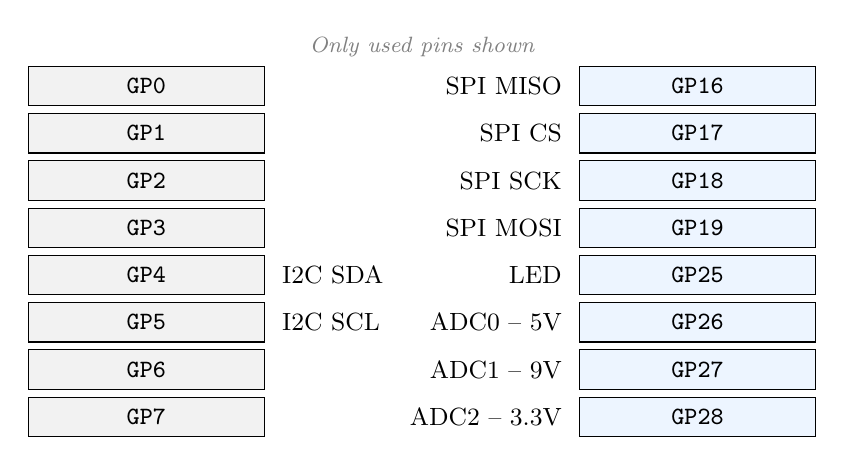
\begin{tikzpicture}[
    pin/.style={draw, minimum width=3cm, minimum height=0.5cm, font=\small\ttfamily},
    label/.style={font=\small, anchor=east},
    rlabel/.style={font=\small, anchor=west},
]
% Left side
\foreach \i/\lbl/\fn in {
    0/GP0/{},
    1/GP1/{},
    2/GP2/{},
    3/GP3/{},
    4/GP4/{I2C SDA},
    5/GP5/{I2C SCL},
    6/GP6/{},
    7/GP7/{}
} {
    \node[pin, fill=gray!10] at (0, -\i*0.6) {\lbl};
    \node[rlabel] at (1.6, -\i*0.6) {\fn};
}
% Right side - SPI + ADC
\foreach \i/\lbl/\fn in {
    0/GP16/{SPI MISO},
    1/GP17/{SPI CS},
    2/GP18/{SPI SCK},
    3/GP19/{SPI MOSI},
    4/GP25/{LED},
    5/GP26/{ADC0 -- 5V},
    6/GP27/{ADC1 -- 9V},
    7/GP28/{ADC2 -- 3.3V}
} {
    \node[pin, fill=accentblue!10] at (7, -\i*0.6) {\lbl};
    \node[label] at (5.4, -\i*0.6) {\fn};
}

\node[font=\footnotesize\itshape, text=gray] at (3.5, 0.5) {Only used pins shown};
\end{tikzpicture}

\subsection{Power System}
\label{sec:power}

Three independent voltage rails, each monitored via ADC every frame:

\begin{table}[ht]
\centering
\caption{Voltage rail specifications and thresholds. See \S\ref{sec:troubleshooting-power} for diagnosis.}
\label{tab:voltage-rails}
\begin{tabular}{l c c c c c}
\toprule
\textbf{Rail} & \textbf{Nominal} & \textbf{Min} & \textbf{Max} & \textbf{ADC Pin} & \textbf{Divider} \\
\midrule
3.3\,V (MCU/sensors) & \SI{3.3}{\volt} & \SI{3.0}{\volt} & \SI{3.6}{\volt} & \pin{28} & 1.0 \\
5\,V (servo logic) & \SI{5.0}{\volt} & \SI{4.5}{\volt} & \SI{5.5}{\volt} & \pin{26} & 1.735 \\
9\,V (battery) & \SI{9.0}{\volt} & \SI{8.0}{\volt} & \SI{10.0}{\volt} & \pin{27} & 3.0 \\
\bottomrule
\end{tabular}
\end{table}

\textbf{ADC conversion formula:}
\begin{equation}
V_\text{actual} = \frac{\text{raw}}{65535} \times \SI{3.3}{\volt} \times \text{divider\_ratio}
\label{eq:adc}
\end{equation}

ADC reads require two sequential \texttt{read\_u16()} calls --- the first selects the channel (discarded), the second is the measurement. If \texttt{raw} $\leq 100$, the pin is considered floating and the reading returns \SI{0}{\milli\volt}.

% ══════════════════════════════════════════════════════
\section{Boot Sequence}
\label{sec:boot}
% ══════════════════════════════════════════════════════

\begin{tikzpicture}[
    step/.style={draw, rounded corners, minimum width=10cm, minimum height=0.7cm, font=\small, fill=accentblue!8},
    fail/.style={draw, rounded corners, minimum width=4cm, minimum height=0.7cm, font=\small, fill=accentred!15},
    arr/.style={-{Stealth[length=3mm]}, thick},
    every node/.style={align=center},
]
\node[step] (s1) at (0,0) {1. Check reset cause --- normal, WDT, or soft reset};
\node[step] (s2) at (0,-1) {2. Read crash context from scratch registers \xref{sec:crash-recovery}};
\node[step] (s3) at (0,-2) {3. Validate \file{config.py} --- ranges, pin conflicts};
\node[step] (s4) at (0,-3) {4. Overclock CPU to \SI{200}{\mega\hertz}};
\node[step] (s5) at (0,-4) {5. Init LED (Timer, 25\,ms tick) --- fast blink};
\node[step] (s6) at (0,-5) {6. Start watchdog (5\,s timeout)};
\node[step] (s7) at (0,-6) {7. Mount SD card --- 3 retries (30 on crash reboot)};
\node[step] (s8) at (0,-7) {8. Init barometer --- chip ID, calibration, live read};
\node[step] (s9) at (0,-8) {9. Init power monitor --- read 3 rails, check health};
\node[step] (s10) at (0,-9) {10. Ground calibration --- 50 pressure samples (10 on crash)};
\node[step] (s11) at (0,-10) {11. Init Kalman filter + state machine};
\node[step] (s12) at (0,-11) {12. Open logger --- create flight folder, write metadata};
\node[step, fill=accentgreen!15] (s13) at (0,-12) {13. Enter flight loop at \SI{50}{\hertz} \xref{sec:flight-loop}};

\node[fail] (f1) at (7,-6) {HALT --- solid LED};
\node[fail] (f2) at (7,-7) {HALT --- solid LED};

\draw[arr] (s1) -- (s2);
\draw[arr] (s2) -- (s3);
\draw[arr] (s3) -- (s4);
\draw[arr] (s4) -- (s5);
\draw[arr] (s5) -- (s6);
\draw[arr] (s6) -- (s7);
\draw[arr] (s7) -- (s8);
\draw[arr] (s8) -- (s9);
\draw[arr] (s9) -- (s10);
\draw[arr] (s10) -- (s11);
\draw[arr] (s11) -- (s12);
\draw[arr] (s12) -- (s13);

\draw[-{Stealth}, dashed, accentred] (s7.east) -- node[above, font=\tiny] {SD fail} (f1.west);
\draw[-{Stealth}, dashed, accentred] (s8.east) -- node[above, font=\tiny] {Baro fail} (f2.west);
\end{tikzpicture}

\textbf{Crash reboot path:} If the reset cause is WDT (value 3) and valid crash data exists in scratch registers, the system skips the full preflight: SD mount gets 30 retries, ground calibration uses 10 samples instead of 50, and a crash report is written to the new flight folder. Total recovery time: $\sim$\SI{0.5}{\second}.

\textbf{Manual override:} If \file{/sd/\_manual\_override} exists, non-critical warnings are bypassed and the 10-second countdown is skipped. The file is deleted after reading.

% ══════════════════════════════════════════════════════
\section{Flight Loop}
\label{sec:flight-loop}
% ══════════════════════════════════════════════════════

\subsection{Timing and Pipeline}
\label{sec:pipeline}

The main loop runs at \SI{50}{\hertz} (\SI{20}{\milli\second} per frame). Timing is enforced by a spin-wait on \texttt{time.ticks\_us()}.

\begin{figure}[ht]
\centering
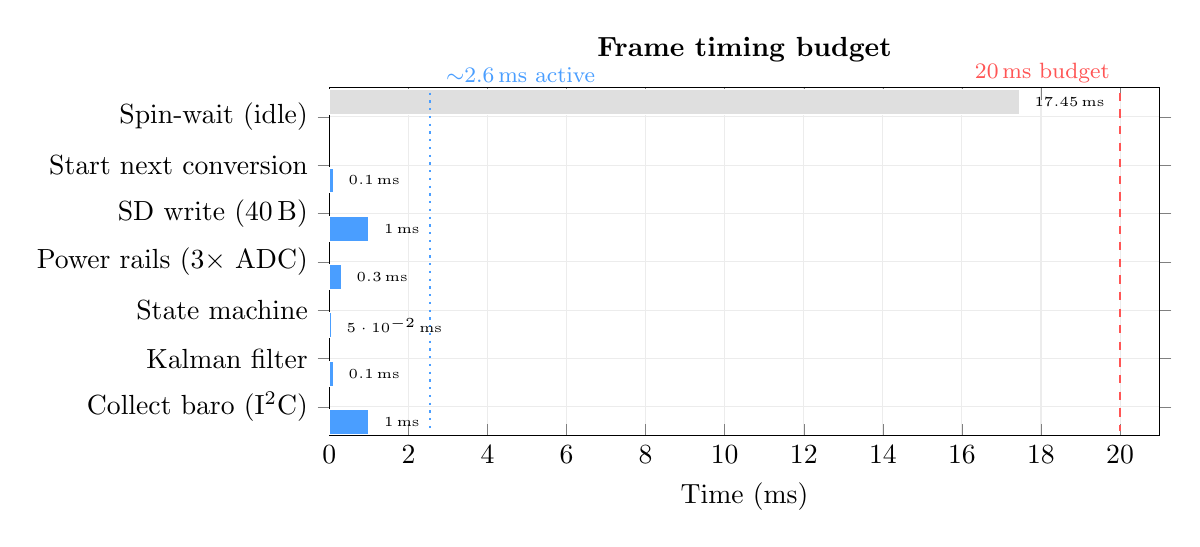
\begin{tikzpicture}
\begin{axis}[
    xbar,
    width=\textwidth,
    height=6cm,
    bar width=9pt,
    xlabel={Time (ms)},
    xmin=0, xmax=21,
    ytick={0,1,2,3,4,5,6},
    yticklabels={
        {Spin-wait (idle)},
        {Start next conversion},
        {SD write (40\,B)},
        {Power rails (3$\times$ ADC)},
        {State machine},
        {Kalman filter},
        {Collect baro (I\textsuperscript{2}C)}
    },
    y dir=reverse,
    grid=major, grid style={gray!15},
    title={\textbf{Frame timing budget}},
    nodes near coords={\pgfmathprintnumber\pgfplotspointmeta\,ms},
    nodes near coords style={font=\tiny, anchor=west, xshift=2pt},
    clip=false,
]
\addplot[fill=accentblue, draw=white] coordinates {(1.0,6)(0.1,5)(0.05,4)(0.3,3)(1.0,2)(0.1,1)};
\addplot[fill=gray!25, draw=white] coordinates {(17.45,0)};

\draw[accentred, dashed, thick] (axis cs:20,-0.5) -- (axis cs:20,6.5)
    node[pos=0.0, anchor=south east, font=\footnotesize] {\SI{20}{\milli\second} budget};
\draw[accentblue, dotted, thick] (axis cs:2.55,-0.5) -- (axis cs:2.55,6.5)
    node[pos=0.0, anchor=south west, font=\footnotesize, xshift=2pt] {$\sim$\SI{2.6}{\milli\second} active};
\end{axis}
\end{tikzpicture}
\caption{Per-stage timing breakdown. Blue = active CPU work. Grey = idle spin-wait while BMP180 ADC converts.}
\label{fig:timing}
\end{figure}

\subsection{Per-Frame Operations}

Each frame executes these steps sequentially:

\begin{enumerate}
    \item \textbf{Collect barometer result} --- I\textsuperscript{2}C read of previous frame's conversion ($\sim$\SI{1}{\milli\second})
    \item \textbf{Compensate} --- apply BMP180 calibration coefficients to raw pressure/temperature
    \item \textbf{Kalman filter update} --- predict + correct cycle \xref{sec:kalman}
    \item \textbf{State machine update} --- evaluate transition conditions \xref{sec:fsm}
    \item \textbf{Read power rails} --- 3$\times$ ADC reads ($\sim$\SI{0.3}{\milli\second})
    \item \textbf{Build flags byte} --- bit 3 set if SD card has failed
    \item \textbf{Write binary frame} --- 40\,B to SD via \texttt{file.write()} ($\sim$\SI{1}{\milli\second})
    \item \textbf{Start next conversion} --- I\textsuperscript{2}C write to kick off BMP180 ADC
    \item \textbf{Feed watchdog}
    \item \textbf{Spin-wait} --- idle until \SI{20}{\milli\second} frame budget expires
\end{enumerate}

\textbf{Slow diagnostics} (once per second): \texttt{gc.collect()}, \texttt{gc.mem\_free()}, CPU temperature from ADC4. These values are reused across frames until next update.

\textbf{Temperature re-read:} BMP180 temperature is re-read every $\sim$\SI{1}{\second} (every \config{SAMPLE\_RATE\_HZ} frames). This is a blocking \SI{5}{\milli\second} read.

\subsection{Error Handling in the Loop}

All exceptions in the sensor loop are caught. On error:
\begin{itemize}
    \item Increment \texttt{\_i2c\_errors} counter (u8, wraps at 255)
    \item Write an error frame: altitude/velocity fields zeroed, \texttt{flags = 0x08}
    \item Continue to next frame --- \textbf{the loop never crashes}
\end{itemize}

% ══════════════════════════════════════════════════════
\section{BMP180 Barometer}
\label{sec:barometer}
% ══════════════════════════════════════════════════════

\subsection{Register Map}
\label{sec:baro-registers}

\begin{table}[ht]
\centering
\caption{BMP180 I\textsuperscript{2}C register addresses.}
\label{tab:bmp180-regs}
\begin{tabular}{l l l}
\toprule
\textbf{Address} & \textbf{Name} & \textbf{Purpose} \\
\midrule
\reg{D0} & REG\_ID & Chip ID --- expect \hex{55} \\
\reg{E0} & REG\_RESET & Soft reset --- write \hex{B6} \\
\reg{F4} & REG\_CTRL\_MEAS & Measurement command register \\
\reg{F6} & REG\_OUT\_MSB & Output data (MSB/LSB/XLSB) \\
\reg{AA} & REG\_CALIB & Calibration data start (22 bytes, big-endian) \\
\bottomrule
\end{tabular}
\end{table}

\subsection{Calibration Coefficients}

Read from EEPROM at \reg{AA}, 22 bytes, big-endian:

\begin{table}[ht]
\centering
\caption{BMP180 calibration coefficients.}
\label{tab:bmp180-cal}
\begin{tabular}{c l l l}
\toprule
\textbf{Offset} & \textbf{Name} & \textbf{Type} & \textbf{Format} \\
\midrule
0 & AC1 & signed & \texttt{>h} \\
2 & AC2 & signed & \texttt{>h} \\
4 & AC3 & signed & \texttt{>h} \\
6 & AC4 & unsigned & \texttt{>H} \\
8 & AC5 & unsigned & \texttt{>H} \\
10 & AC6 & unsigned & \texttt{>H} \\
12 & B1 & signed & \texttt{>h} \\
14 & B2 & signed & \texttt{>h} \\
16 & MB & signed & \texttt{>h} \\
18 & MC & signed & \texttt{>h} \\
20 & MD & signed & \texttt{>h} \\
\bottomrule
\end{tabular}
\end{table}

\textbf{Sanity check:} If AC1 $= 0$ or AC1 $= \texttt{0xFFFF}$, the EEPROM is blank or corrupted.

\subsection{Compensation Formulas}

\textbf{Temperature} (from raw UT):
\begin{align}
X_1 &= \frac{(\text{UT} - \text{AC6}) \times \text{AC5}}{2^{15}} \\
X_2 &= \frac{\text{MC} \times 2^{11}}{X_1 + \text{MD}} \\
B_5 &= X_1 + X_2 \\
T &= \frac{B_5 + 8}{160} \quad [\si{\degreeCelsius}]
\end{align}

\textbf{Pressure} (from raw UP, using $B_5$ from temperature, OSS=2): the full Bosch compensation algorithm is implemented in \file{sensors/barometer.py}. The result is pressure in Pascals.

\textbf{Altitude} (hypsometric formula):
\begin{equation}
h = 44330 \times \left(1 - \left(\frac{P}{P_\text{ground}}\right)^{0.1903}\right) \quad [\si{\metre}]
\label{eq:altitude}
\end{equation}

where $P_\text{ground}$ is the baseline pressure from ground calibration \xref{sec:boot}.

\subsection{Pipelined Read API}

\begin{enumerate}
    \item \texttt{baro.start(temp=False)} --- writes command to \reg{F4}, sets \texttt{\_pending}. Call at frame end.
    \item \texttt{baro.collect()} --- reads result from \reg{F6} (no sleep). Call at next frame start.
    \item \texttt{baro.compensate(UT, UP)} --- applies calibration. Returns \texttt{(pressure\_pa, temperature\_c)}.
\end{enumerate}

\textbf{Conversion times:} OSS\,0 = \SI{5}{\milli\second}, OSS\,1 = \SI{8}{\milli\second}, OSS\,2 = \SI{14}{\milli\second}, OSS\,3 = \SI{26}{\milli\second}. We use OSS\,=\,2 (\SI{13.5}{\milli\second} typical).

% ══════════════════════════════════════════════════════
\section{Kalman Filter}
\label{sec:kalman}
% ══════════════════════════════════════════════════════

\subsection{State Model}

State vector $\mathbf{x} = [\text{altitude},\; \text{velocity}]^\top$. Constant-velocity process model:

\begin{equation}
\mathbf{F} = \begin{bmatrix} 1 & \Delta t \\ 0 & 1 \end{bmatrix}, \quad
\mathbf{H} = \begin{bmatrix} 1 & 0 \end{bmatrix}, \quad
\mathbf{Q} = \begin{bmatrix} q_\text{alt} & 0 \\ 0 & q_\text{vel} \end{bmatrix}
\end{equation}

\subsection{Tuning Parameters}

\begin{table}[ht]
\centering
\caption{Kalman filter noise parameters. Adjust in \file{config.py}.}
\label{tab:kalman-params}
\begin{tabular}{l l l l}
\toprule
\textbf{Parameter} & \textbf{Config key} & \textbf{Default} & \textbf{Effect of increase} \\
\midrule
$q_\text{alt}$ & \config{KALMAN\_Q\_ALT} & 0.1\,m$^2$ & Noisier altitude, faster response \\
$q_\text{vel}$ & \config{KALMAN\_Q\_VEL} & 0.5\,m$^2$/s$^2$ & Noisier velocity, faster response \\
$R$ & \config{KALMAN\_R\_ALT} & 1.0\,m$^2$ & Trust model more, trust barometer less \\
\bottomrule
\end{tabular}
\end{table}

\subsection{Predict Step}
\begin{align}
\hat{x}_\text{alt} &= x_\text{alt} + x_\text{vel} \cdot \Delta t \\
\hat{x}_\text{vel} &= x_\text{vel} \\
\hat{P}_{00} &= P_{00} + \Delta t \,(P_{10} + P_{01}) + \Delta t^2\, P_{11} + q_\text{alt} \\
\hat{P}_{01} &= P_{01} + \Delta t\, P_{11}, \quad \hat{P}_{10} = P_{10} + \Delta t\, P_{11}, \quad \hat{P}_{11} = P_{11} + q_\text{vel}
\end{align}

\subsection{Update Step}
\begin{align}
y &= z - \hat{x}_\text{alt} \quad \text{(innovation)} \\
S &= \hat{P}_{00} + R \\
K_0 &= \hat{P}_{00} / S, \quad K_1 = \hat{P}_{10} / S \\
x_\text{alt} &= \hat{x}_\text{alt} + K_0 \cdot y \\
x_\text{vel} &= \hat{x}_\text{vel} + K_1 \cdot y
\end{align}

\textbf{Safeguards:} If $|S| < 10^{-10}$, skip the update (degenerate). Diagonal of $P$ is clamped $\geq 0$ to prevent negative variance from rounding.

\textbf{Initialisation:} The filter is primed with 20 barometer readings before the flight loop begins. First call to \texttt{update()} without prior \texttt{reset()} auto-initialises with the measured altitude.

% ══════════════════════════════════════════════════════
\section{Flight State Machine}
\label{sec:fsm}
% ══════════════════════════════════════════════════════

\subsection{State Definitions}

\begin{table}[ht]
\centering
\caption{Flight states. All states are logged only --- no deployment hardware on this board.}
\label{tab:states}
\begin{tabular}{c l l}
\toprule
\textbf{Value} & \textbf{State} & \textbf{Description} \\
\midrule
0 & \state{pad} & On launch pad, waiting \\
1 & \state{boost} & Motor burning, ascending \\
2 & \state{coast} & Motor out, still ascending \\
3 & \state{apogee} & Peak altitude reached \\
4 & \state{drogue} & Under drogue chute, initial descent \\
5 & \state{main} & Under main chute, final descent \\
6 & \state{landed} & On ground, flight complete \\
\bottomrule
\end{tabular}
\end{table}

\subsection{Transition Conditions}
\label{sec:fsm-transitions}

All thresholds are configurable in \file{config.py}. Default values shown.

\begin{table}[ht]
\centering
\small
\caption{State transition logic and thresholds.}
\label{tab:transitions}
\begin{tabularx}{\textwidth}{l l X l}
\toprule
\textbf{From} & \textbf{To} & \textbf{Condition} & \textbf{Threshold} \\
\midrule
\state{pad} & \state{boost} & AGL $>$ \config{LAUNCH\_ALT} \textbf{and} vel $>$ \config{LAUNCH\_VEL}, sustained for \config{LAUNCH\_DETECT\_WINDOW} & 15\,m, 10\,m/s, 0.5\,s \\
\state{boost} & \state{pad} & Within \config{BOOST\_RECOVERY\_WINDOW} of launch \textbf{and} AGL $<$ \config{BOOST\_RECOVERY\_ALT} for \config{BOOST\_RECOVERY\_COUNT} frames & 2\,s, 10\,m, 3 frames \\
\state{boost} & \state{coast} & vel $<$ (max\_vel $-$ \config{COAST\_VEL\_THRESHOLD}) & 5\,m/s drop \\
\state{coast} & \state{apogee} & vel $<$ \config{APOGEE\_VEL} for \config{APOGEE\_CONFIRM\_COUNT} frames, \textbf{or} \config{COAST\_TIMEOUT} elapsed & 2\,m/s, 5 frames, 30\,s \\
\state{apogee} & \state{drogue} & Dwell for \config{APOGEE\_DWELL\_FRAMES} frames & 5 frames \\
\state{drogue} & \state{main} & AGL $\leq$ max\_AGL $\times$ \config{MAIN\_CHUTE\_FRACTION} \textbf{and} vel $< 0$ & 25\% \\
\state{drogue}/\state{main} & \state{landed} & $|\text{vel}| <$ \config{LANDED\_VEL} for \config{LANDED\_CONFIRM\_SECONDS} & 0.5\,m/s, 5\,s \\
\bottomrule
\end{tabularx}
\end{table}

\subsection{State Diagram}

\begin{figure}[ht]
\centering
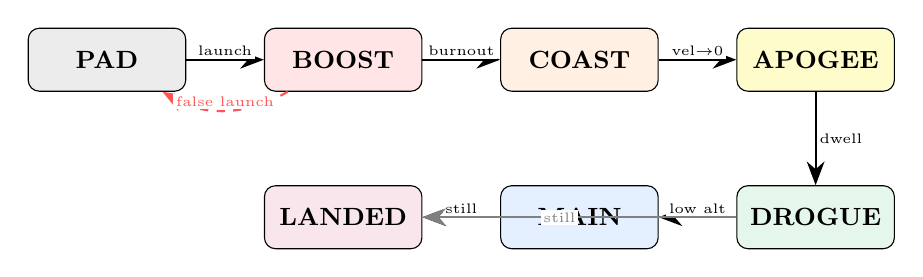
\begin{tikzpicture}[
    state/.style={draw, rounded corners, minimum width=2cm, minimum height=0.8cm, font=\small\bfseries},
    arr/.style={-{Stealth[length=3mm]}, thick},
    cond/.style={font=\tiny, fill=white, inner sep=1pt},
]
\node[state, fill=gray!15] (pad) at (0,0) {PAD};
\node[state, fill=accentred!15] (boost) at (3,0) {BOOST};
\node[state, fill=accentorange!15] (coast) at (6,0) {COAST};
\node[state, fill=yellow!20] (apogee) at (9,0) {APOGEE};
\node[state, fill=accentgreen!15] (drogue) at (9,-2) {DROGUE};
\node[state, fill=accentblue!15] (main) at (6,-2) {MAIN};
\node[state, fill=purple!10] (landed) at (3,-2) {LANDED};

\draw[arr] (pad) -- node[cond, above] {launch} (boost);
\draw[arr, dashed, accentred] (boost) to[bend left=30] node[cond, above] {false launch} (pad);
\draw[arr] (boost) -- node[cond, above] {burnout} (coast);
\draw[arr] (coast) -- node[cond, above] {vel$\to$0} (apogee);
\draw[arr] (apogee) -- node[cond, right] {dwell} (drogue);
\draw[arr] (drogue) -- node[cond, above] {low alt} (main);
\draw[arr] (main) -- node[cond, above] {still} (landed);
\draw[arr, gray] (drogue) -- node[cond, left, text=gray] {still} (landed);
\end{tikzpicture}
\caption{Flight state transitions. Dashed line = false launch recovery path.}
\label{fig:fsm}
\end{figure}

% ══════════════════════════════════════════════════════
\section{Binary Log Format (V3)}
\label{sec:log-format}
% ══════════════════════════════════════════════════════

\subsection{File Structure}

\begin{lstlisting}[caption={SD card file layout per flight.}]
/sd/flight_NNN/
    flight.bin       Binary telemetry frames
    preflight.txt    Boot metadata, voltages, config
    boot.txt         Full serial output during boot
    crash.txt        Previous WDT crash report (if applicable)
\end{lstlisting}

\textbf{File header} (10 bytes): \texttt{b'RKTLOG'} (6\,B) $+$ version u16 LE (= 3) $+$ frame\_size u16 LE (= 40).

\textbf{Each frame}: 2-byte sync header \texttt{0xAA\,0x55} $+$ 40-byte data.

\subsection{Frame Layout}
\label{sec:frame-layout}

Struct format: \texttt{<IBfffffHHHBHHBBBB} (40 bytes, little-endian).

\begin{table}[ht]
\centering
\small
\caption{V3 binary frame fields. All multi-byte values are little-endian.}
\label{tab:frame-v3}
\begin{tabular}{c l l c l}
\toprule
\textbf{Offset} & \textbf{Field} & \textbf{Type} & \textbf{Bytes} & \textbf{Notes} \\
\midrule
0 & timestamp\_ms & u32 & 4 & Milliseconds since boot \\
4 & state & u8 & 1 & Flight state 0--6 \xref{sec:fsm} \\
5 & pressure\_pa & f32 & 4 & Raw barometric pressure \\
9 & temperature\_c & f32 & 4 & Sensor temperature \\
13 & alt\_raw\_m & f32 & 4 & Unfiltered altitude AGL \\
17 & alt\_filtered\_m & f32 & 4 & Kalman-filtered altitude \\
21 & vel\_filtered\_ms & f32 & 4 & Kalman-filtered velocity \\
25 & v\_3v3\_mv & u16 & 2 & 3.3\,V rail \xref{sec:power} \\
27 & v\_5v\_mv & u16 & 2 & 5\,V rail \\
29 & v\_9v\_mv & u16 & 2 & 9\,V battery rail \\
31 & flags & u8 & 1 & Status flags (see below) \\
32 & frame\_us & u16 & 2 & Frame execution time \\
34 & flush\_us & u16 & 2 & Last SD flush duration \\
36 & free\_kb & u8 & 1 & Heap free $\div$ 1024 \\
37 & cpu\_temp\_c & u8 & 1 & CPU temp $+$ 40 offset \\
38 & i2c\_errors & u8 & 1 & Cumulative (wraps 255) \\
39 & overruns & u8 & 1 & Loop overruns (wraps 255) \\
\bottomrule
\end{tabular}
\end{table}

\subsection{Flags Byte}
\label{sec:flags}

\begin{table}[ht]
\centering
\caption{Flags byte bit assignments.}
\label{tab:flags}
\begin{tabular}{c l l}
\toprule
\textbf{Bit} & \textbf{Name} & \textbf{Meaning} \\
\midrule
0 & \texttt{ARMED} & Flight computer armed and logging \\
1 & \texttt{DROGUE\_FIRED} & Drogue deployment event detected \\
2 & \texttt{MAIN\_FIRED} & Main deployment event detected \\
3 & \texttt{ERROR} & SD write failure or I\textsuperscript{2}C fault \\
4--7 & --- & Reserved \\
\bottomrule
\end{tabular}
\end{table}

A frame with no flags set decodes as \texttt{SAFE}.

\subsection{Version History}
\label{sec:format-versions}

\begin{table}[ht]
\centering
\caption{Binary format evolution.}
\label{tab:versions}
\begin{tabular}{l c c c}
\toprule
& \textbf{V1} & \textbf{V2} & \textbf{V3} \\
\midrule
Frame size & 28\,B & 32\,B & 40\,B \\
Struct format & \texttt{<IBfffffHB} & \texttt{<IBfffffHHHB} & \texttt{<IBfffffHHHBHHBBBB} \\
Voltage rails & 1 (battery) & 3 (3.3/5/9\,V) & 3 (3.3/5/9\,V) \\
Diagnostics & None & None & 6 fields \\
Sample rate & \SI{25}{\hertz} & \SI{25}{\hertz} & \SI{50}{\hertz} \\
Throughput & \SI{700}{B/s} & \SI{800}{B/s} & \SI{2000}{B/s} \\
Crash recovery & No & No & Yes \\
\bottomrule
\end{tabular}
\end{table}

\subsection{Flush Strategy}
\label{sec:flush}

\begin{itemize}
    \item \textbf{Every \config{LOG\_FLUSH\_EVERY} frames} (default 50, $\approx$\SI{1}{\second}): \texttt{file.flush()}, write crash context to scratch registers, feed watchdog
    \item \textbf{Every \config{LOG\_SYNC\_EVERY} flushes} (default 3, $\approx$\SI{3}{\second}): \texttt{os.sync()} to commit FAT metadata
    \item \textbf{On state transition}: immediate flush $+$ sync
\end{itemize}

Flush duration is measured in microseconds and logged in the \textit{next} frame's \texttt{flush\_us} field.

% ══════════════════════════════════════════════════════
\section{Crash Recovery}
\label{sec:crash-recovery}
% ══════════════════════════════════════════════════════

\subsection{Watchdog Scratch Registers}

The RP2040 watchdog peripheral has scratch registers that survive a WDT reset:

\begin{table}[ht]
\centering
\caption{Scratch register layout.}
\label{tab:scratch}
\begin{tabular}{l l l}
\toprule
\textbf{Address} & \textbf{Register} & \textbf{Contents} \\
\midrule
\texttt{0x40058024} & SCRATCH6 & \texttt{0xDEAD} (bits 31--16) | frame\_count (bits 15--0) \\
\texttt{0x40058028} & SCRATCH7 & timestamp\_ms (32 bits) \\
\bottomrule
\end{tabular}
\end{table}

\textbf{Written:} before every flush in \texttt{write\_scratch()}.\\
\textbf{Read:} at boot in \texttt{read\_crash\_report()}. Valid if upper 16 bits of SCRATCH6 $=$ \hex{DEAD}.

\subsection{Recovery Flow}

\begin{enumerate}
    \item RP2040 resets (WDT timeout or brown-out)
    \item \texttt{reset\_cause()} returns 3 (WDT\_RESET)
    \item Read SCRATCH6/7 --- extract frame count, timestamp
    \item Fast boot: mount SD (30 retries), calibrate (10 samples)
    \item Write \file{crash.txt} to new flight folder with: reboot reason, frame count, timestamp, state, flags, CPU temp
    \item Resume logging in $\sim$\SI{0.5}{\second}
\end{enumerate}

\subsection{SD Card Recovery}
\label{sec:sd-recovery}

If an SD write fails (\texttt{OSError}), the frame is retried once. If it fails again:
\begin{itemize}
    \item \texttt{sd\_failed} flag is set (logged as \texttt{flags |= 0x08})
    \item Sensor loop continues running
    \item Every \SI{5}{\second}: \texttt{try\_recover()} closes the broken file, creates a new flight folder, opens a new \file{flight.bin}
    \item Data already written to the previous file is preserved
\end{itemize}

% ══════════════════════════════════════════════════════
\section{LED Status Patterns}
\label{sec:led}
% ══════════════════════════════════════════════════════

Driven by hardware Timer(-1) with a \SI{25}{\milli\second} tick as a soft IRQ callback. No \texttt{\_thread}, no GIL contention.

\begin{table}[ht]
\centering
\caption{LED blink patterns by state. Each value is a duration in milliseconds; the LED toggles after each.}
\label{tab:led}
\begin{tabular}{l l l}
\toprule
\textbf{State/Condition} & \textbf{Pattern (ms)} & \textbf{Visual} \\
\midrule
\state{pad} (ready) & [1000, 1000] & Slow blink \\
\state{boost} & [50, 50] & Rapid flash \\
\state{coast} & [100, 100] & Medium blink \\
\state{apogee} & [100, 100, 100, 500] & Double flash \\
\state{drogue} & [200, 200] & Medium-fast \\
\state{main} & [300, 300] & Medium \\
\state{landed} & [100, 100, 100, 100, 100, 800] & Triple flash \\
Preflight running & [250, 250] & Fast blink \\
Error / HALT & Solid ON & Continuous \\
\bottomrule
\end{tabular}
\end{table}

% ══════════════════════════════════════════════════════
\section{Configuration Reference}
\label{sec:config}
% ══════════════════════════════════════════════════════

All tuneable values live in \file{config.py}. The firmware calls \texttt{config.validate()} at boot to check ranges and pin conflicts.

\begin{longtable}{l l l p{5.5cm}}
\caption{Complete configuration reference.} \label{tab:config} \\
\toprule
\textbf{Key} & \textbf{Default} & \textbf{Unit} & \textbf{Notes} \\
\midrule
\endfirsthead
\toprule
\textbf{Key} & \textbf{Default} & \textbf{Unit} & \textbf{Notes} \\
\midrule
\endhead
\multicolumn{4}{l}{\textit{Software}} \\
VERSION & 1.16.0 & --- & Semantic version string \\
\midrule
\multicolumn{4}{l}{\textit{I\textsuperscript{2}C (Barometer)}} \\
I2C\_SDA & 4 & GPIO & BMP180 data line \\
I2C\_SCL & 5 & GPIO & BMP180 clock line \\
I2C\_FREQ & 100\,000 & Hz & SoftI2C frequency \\
I2C\_TIMEOUT\_US & 50\,000 & $\mu$s & I\textsuperscript{2}C timeout \\
BMP180\_ADDR & 0x77 & hex & I\textsuperscript{2}C address \\
\midrule
\multicolumn{4}{l}{\textit{SPI (SD Card)}} \\
SPI\_ID & 0 & --- & Hardware SPI peripheral \\
SPI\_MISO & 16 & GPIO & \\
SPI\_CS & 17 & GPIO & \\
SPI\_SCK & 18 & GPIO & \\
SPI\_MOSI & 19 & GPIO & \\
SPI\_BAUD & 10\,000\,000 & Hz & Operating baudrate \\
\midrule
\multicolumn{4}{l}{\textit{ADC (Power Monitoring)}} \\
ADC\_V5 & 26 & GPIO & 5\,V rail \\
ADC\_V9 & 27 & GPIO & 9\,V rail \\
ADC\_V3 & 28 & GPIO & 3.3\,V rail \\
VREF & 3.3 & V & ADC reference voltage \\
ADC\_RESOLUTION & 65535 & counts & 16-bit scaled \\
VDIV\_3V & 1.0 & ratio & No divider \\
VDIV\_5V & 1.735 & ratio & 500$\Omega$/680$\Omega$ \\
VDIV\_9V & 3.0 & ratio & 2\,k$\Omega$/1\,k$\Omega$ \\
\midrule
\multicolumn{4}{l}{\textit{Logging}} \\
SAMPLE\_RATE\_HZ & 50 & Hz & Main loop rate (1--100) \\
LOG\_FLUSH\_EVERY & 50 & frames & Flush interval \\
LOG\_SYNC\_EVERY & 3 & flushes & FAT sync interval \\
GROUND\_SAMPLES & 50 & samples & Pressure calibration \\
BARO\_AVG\_EXTRA & 1 & reads & Extra averaging \\
\midrule
\multicolumn{4}{l}{\textit{Kalman Filter}} \\
KALMAN\_Q\_ALT & 0.1 & m$^2$ & Altitude process noise \\
KALMAN\_Q\_VEL & 0.5 & m$^2$/s$^2$ & Velocity process noise \\
KALMAN\_R\_ALT & 1.0 & m$^2$ & Measurement noise \\
\midrule
\multicolumn{4}{l}{\textit{State Machine --- see Table~\ref{tab:transitions} for usage}} \\
LAUNCH\_ALT\_THRESHOLD & 15.0 & m & \\
LAUNCH\_VEL\_THRESHOLD & 10.0 & m/s & \\
LAUNCH\_DETECT\_WINDOW & 0.5 & s & \\
BOOST\_RECOVERY\_ALT & 10.0 & m & \\
BOOST\_RECOVERY\_WINDOW & 2.0 & s & \\
BOOST\_RECOVERY\_COUNT & 3 & frames & \\
COAST\_VEL\_THRESHOLD & 5.0 & m/s & \\
COAST\_TIMEOUT & 30.0 & s & \\
APOGEE\_VEL\_THRESHOLD & 2.0 & m/s & \\
APOGEE\_CONFIRM\_COUNT & 5 & frames & \\
APOGEE\_DWELL\_FRAMES & 5 & frames & \\
MAIN\_CHUTE\_FRACTION & 0.25 & ratio & \\
LANDED\_VEL\_THRESHOLD & 0.5 & m/s & \\
LANDED\_CONFIRM\_SECONDS & 5.0 & s & \\
\midrule
\multicolumn{4}{l}{\textit{Hardware}} \\
LED\_PIN & 25 & GPIO & Onboard LED \\
\bottomrule
\end{longtable}

% ══════════════════════════════════════════════════════
\section{Diagnostic Suite}
\label{sec:diagnostics}
% ══════════════════════════════════════════════════════

Eight tests run directly on the Pico via USB (\texttt{pnpm pico:diag}). Each exercises a specific subsystem in isolation.

\begin{table}[ht]
\centering
\small
\caption{Diagnostic test suite. Run via \texttt{pnpm pico:diag} or \texttt{import pico\_diag; pico\_diag.menu()}.}
\label{tab:diag}
\begin{tabularx}{\textwidth}{c l c c X}
\toprule
\textbf{\#} & \textbf{Test} & \textbf{Time} & \textbf{HW?} & \textbf{What it measures} \\
\midrule
1 & Sensor Bench & 40\,s & Yes & 1000 baro reads: I\textsuperscript{2}C latency histogram, pressure noise, clock stretch \\
2 & SD Card Bench & 330\,s & Yes & Burst + 5\,min sustained writes: per-frame/flush latency, error rate \\
3 & Loop Budget & 45\,s & Yes & Per-stage timing: baro, altitude, Kalman, FSM, power, struct pack \\
4 & RAM Profile & 60\,s & Yes & Object memory cost + 1000-frame leak detection ($\leq$100\,B = pass) \\
5 & Float Precision & 15\,s & No & 10k Kalman iterations: constant drift ($<$0.1\,m), ramp tracking, covariance \\
6 & Dual-Core Stress & 70\,s & Yes & Core\,0 jitter with/without Timer LED. Max frame time vs budget \\
7 & Endurance Run & 600\,s & Yes & 10\,min pipeline: 30\,s snapshots of timing drift, RAM, temp, errors \\
8 & Error Injection & 30\,s & Yes & Bad I\textsuperscript{2}C, SD removal, extreme Kalman/FSM inputs: graceful recovery \\
\bottomrule
\end{tabularx}
\end{table}

\textbf{Sensor bench histogram bins} ($\mu$s): 25000, 28000, 30000, 32000, 34000, 36000, 38000, 40000, 50000, 100000.

\textbf{Pressure-to-altitude noise}: $\sigma_\text{alt} \approx \sigma_P \times 0.083$\,m/Pa.

\textbf{RAM leak threshold}: $\leq$100\,bytes per 1000 frames = negligible.

\textbf{Endurance stability criteria}: timing drift $<$\SI{500}{\micro\second}, RAM change $<$200\,B, temp drift $<$\SI{5}{\degreeCelsius}, zero errors.

% ══════════════════════════════════════════════════════
\section{Ground Station Tools}
\label{sec:tools}
% ══════════════════════════════════════════════════════

\begin{table}[ht]
\centering
\caption{Laptop-side tools and their pnpm commands.}
\label{tab:tools}
\begin{tabularx}{\textwidth}{l l X}
\toprule
\textbf{Command} & \textbf{Script} & \textbf{Purpose} \\
\midrule
\texttt{pnpm preflight} & \file{tools/preflight.py} & Step-by-step checklist with GO/NO-GO + live telemetry \\
\texttt{pnpm postflight} & \file{tools/postflight.py} & Download log, decode, display metrics + diagnostics \\
\texttt{pnpm pico:diag} & \file{tools/pico\_diag\_tui.py} & Remote diagnostic test suite \xref{sec:diagnostics} \\
\texttt{pnpm restate} & \file{tools/restate.py} & Offline state machine replay with tuneable thresholds \\
\texttt{pnpm simulator} & \file{tools/simulate.py} & 1D flight prediction with motor database \\
\texttt{pnpm decode} & \file{tools/decode\_log.py} & Binary $\to$ CSV + matplotlib plots \\
\texttt{pnpm deploy:pico} & --- & Flash firmware to Pico \\
\bottomrule
\end{tabularx}
\end{table}

\subsection{Preflight Checklist}
Connects via USB serial (115200 baud, raw REPL). Tames the watchdog by re-initialising with \SI{8300}{\milli\second} timeout and a \SI{2}{\second} Timer feed. Checks: I\textsuperscript{2}C scan, barometer chip ID, SD mount + write test, 3 voltage rails, LED. Provides live Kalman-filtered altitude and velocity monitoring. Issues GO/NO-GO.

\subsection{Postflight Analysis}
Downloads binary log from Pico (or reads from SD card at \texttt{/Volumes/AVIONICS/}). Decodes all three format versions with automatic detection. Computes: max altitude, max velocity, state transition timeline, deployment events. V3 diagnostics: frame timing sparklines, heap trending (leak detection at $-$10\,KB), CPU temp, flush latency (SD stall $>$\SI{50}{\micro\second}), I\textsuperscript{2}C errors, overruns.

\subsection{State Reprocessor}
Replays recorded altitude and velocity through a configurable offline state machine. All thresholds adjustable via CLI args. Produces side-by-side comparison of onboard vs.\ reprocessed states. Can patch binary files in-place or export CSV.

\subsection{Log Decoder}
Searches byte-by-byte for \texttt{0xAA\,0x55} sync headers to align frames (handles corruption). Exports CSV with all fields plus \texttt{state\_name} and \texttt{flags\_str} columns. Optional 4-panel matplotlib plot: altitude (raw + filtered), velocity, pressure, power rails.

% ══════════════════════════════════════════════════════
\section{Preflight and Postflight Checks}
\label{sec:checks}
% ══════════════════════════════════════════════════════

\subsection{hw\_check.py --- Standalone Hardware Test}
\label{sec:hwcheck}

Run on bare Pico with no dependencies. Six tests:

\begin{enumerate}
    \item \textbf{LED}: Blink 5$\times$ (200\,ms on/off). Visual pass.
    \item \textbf{I\textsuperscript{2}C scan}: Scan \hex{00}--\hex{7F}. Pass: $\geq$1 device. Known: \hex{77} = BMP180, \hex{68}/\hex{69} = MPU6050.
    \item \textbf{BMP180}: Chip ID = \hex{55}, calibration non-zero, temp in $-$40--85\si{\degreeCelsius}, 10-sample pressure noise $<$200 LSB.
    \item \textbf{ADC rails}: 3.3\,V [3.0--3.6], 5\,V [3.0--7.0], 9\,V [5.0--12.0].
    \item \textbf{SD card}: Mount, write/read round-trip, free space report, cleanup.
    \item \textbf{Timing}: 100 BMP180 read cycles. Max time vs.\ frame budget at target sample rate.
\end{enumerate}

\subsection{ground\_test.py --- Pad Verification}
\label{sec:groundtest}

Quick pre-flight check on the pad: CPU freq (200\,MHz), SD mount + free space, 10-sample barometer (80--110\,kPa), power rails, LED, 100-cycle timing test. Prints \texttt{ALL CHECKS PASSED --- READY FOR FLIGHT} or error summary.

% ══════════════════════════════════════════════════════
\section{Troubleshooting}
\label{sec:troubleshooting}
% ══════════════════════════════════════════════════════

\subsection{Boot Failures}

\begin{table}[ht]
\centering
\small
\caption{Boot failure symptoms and diagnosis.}
\label{tab:boot-failures}
\begin{tabularx}{\textwidth}{l l X}
\toprule
\textbf{Symptom} & \textbf{LED} & \textbf{Cause / Fix} \\
\midrule
No LED at all & Off & Power not reaching Pico. Check USB, check 3.3\,V rail. \\
Solid LED, no serial & Solid & SD card or barometer failed preflight. Connect serial to see which step failed. Check SD card is inserted and formatted FAT32. Check BMP180 wiring (SDA = \pin{4}, SCL = \pin{5}). \\
Fast blink, never transitions & [250, 250] & Stuck in preflight. Likely waiting for user input or countdown. Check for \file{\_manual\_override} on SD. \\
Repeated reboots & Flickers & Watchdog firing repeatedly. Likely crash in boot sequence. Check \file{crash.txt} in latest flight folder. Run \texttt{pnpm pico:diag} endurance test. \\
\bottomrule
\end{tabularx}
\end{table}

\subsection{Power Issues}
\label{sec:troubleshooting-power}

\begin{table}[ht]
\centering
\small
\caption{Power anomaly diagnosis from log data.}
\label{tab:power-diag}
\begin{tabularx}{\textwidth}{l X}
\toprule
\textbf{Pattern in log} & \textbf{Diagnosis} \\
\midrule
9\,V dips during flush\_us spikes & Battery internal resistance. Normal for alkaline 9\,V under load. Replace if dips below \SI{8}{\volt}. \xref{sec:flush} \\
9\,V steady decline over time & Battery draining. Expect $\sim$\SI{0.5}{\volt} drop per hour for alkaline. \\
3.3\,V drops below \SI{3.0}{\volt} & Regulator overloaded or failing. Check for shorts. \\
5\,V intermittent & Loose connection on buck/boost converter. \\
All rails drop simultaneously & Brown-out. Battery cannot supply peak current (typically during SD flush). \\
\bottomrule
\end{tabularx}
\end{table}

\subsection{Sensor Issues}

\begin{table}[ht]
\centering
\small
\caption{Barometer and I\textsuperscript{2}C diagnosis.}
\label{tab:sensor-diag}
\begin{tabularx}{\textwidth}{l X}
\toprule
\textbf{Symptom} & \textbf{Diagnosis} \\
\midrule
i2c\_errors climbing steadily & Wiring issue, loose connection, or EMI. Check SDA/SCL pull-ups. Run sensor bench \xref{sec:diagnostics}. \\
Altitude noise $>$\SI{2}{\metre} & High pressure noise. Check BMP180 placement (away from airflow). Increase \config{KALMAN\_R\_ALT} for more filtering. \\
Altitude stuck at 0 & Ground calibration used bad pressure. Re-run ground test. Check barometer chip ID with hw\_check. \\
Temperature reads $-$40\si{\degreeCelsius} & I\textsuperscript{2}C read returning all zeros. Bus hung. Power cycle Pico. \\
Pressure out of 80--110\,kPa & Barometer faulty or altitude $>$\SI{2000}{\metre} ASL. Verify with known-good sensor. \\
\bottomrule
\end{tabularx}
\end{table}

\subsection{SD Card Issues}

\begin{table}[ht]
\centering
\small
\caption{SD card diagnosis.}
\label{tab:sd-diag}
\begin{tabularx}{\textwidth}{l X}
\toprule
\textbf{Symptom} & \textbf{Diagnosis} \\
\midrule
\texttt{flags = 0x08} in frames & SD write failed. Check \texttt{flush\_us} for spikes. Card may be full, loose, or damaged. \\
flush\_us $>$ \SI{50}{\milli\second} & Slow SD card. Cards vary widely. Use Class 10 or better. Run SD bench \xref{sec:diagnostics}. \\
Corrupted frames in log & Power loss during write. Decoder resyncs via \texttt{0xAA\,0x55} headers. Frames before corruption are safe. \\
No flight folder created & SD not formatted FAT32, or mount failed silently. Re-format and test with hw\_check. \\
Recovery creates many folders & SD card intermittently failing. \texttt{try\_recover()} opens new folder each time. Card is dying. \\
\bottomrule
\end{tabularx}
\end{table}

\subsection{State Machine Issues}

\begin{table}[ht]
\centering
\small
\caption{Flight state diagnosis. Use \texttt{pnpm restate} to replay with different thresholds.}
\label{tab:fsm-diag}
\begin{tabularx}{\textwidth}{l X}
\toprule
\textbf{Problem} & \textbf{Diagnosis / Fix} \\
\midrule
Never left \state{pad} & Launch thresholds too high, or Kalman filter too sluggish. Lower \config{LAUNCH\_ALT\_THRESHOLD} or \config{KALMAN\_Q\_VEL}. \\
False launch on pad & Thresholds too sensitive. Increase \config{LAUNCH\_ALT\_THRESHOLD} or \config{LAUNCH\_DETECT\_WINDOW}. \\
\state{boost} $\to$ \state{pad} reset & False launch recovery triggered. Check if rocket actually launched. If so, increase \config{BOOST\_RECOVERY\_WINDOW} or lower \config{BOOST\_RECOVERY\_ALT}. \\
Apogee detected too late & \config{APOGEE\_VEL\_THRESHOLD} too low or \config{APOGEE\_CONFIRM\_COUNT} too high. Also check Kalman velocity lag. \\
Stuck in \state{coast} (timeout) & Velocity estimate never reached threshold. Kalman filter too sluggish. Increase \config{KALMAN\_Q\_VEL}. \\
Never reached \state{landed} & \config{LANDED\_VEL\_THRESHOLD} too tight or wind causing motion. Increase threshold or \config{LANDED\_CONFIRM\_SECONDS}. \\
\bottomrule
\end{tabularx}
\end{table}

\subsection{Performance Issues}

\begin{table}[ht]
\centering
\small
\caption{Performance diagnosis from V3 diagnostic fields.}
\label{tab:perf-diag}
\begin{tabularx}{\textwidth}{l X}
\toprule
\textbf{Diagnostic field} & \textbf{What to look for} \\
\midrule
\texttt{frame\_us} $>$ 20000 & Loop overrun. Check what else is running. Run loop budget test. \\
\texttt{overruns} climbing & Sustained overruns. May indicate SD card slowdown or I\textsuperscript{2}C stalls. \\
\texttt{free\_kb} declining & Memory leak. Run RAM profile diagnostic. Should be stable ($\pm$100\,B). \\
\texttt{cpu\_temp\_c} $>$ 70 & Thermal stress. Check ventilation. Value is stored with $+$40 offset (0 = $-$40\si{\degreeCelsius}). \\
\texttt{flush\_us} spikes & SD card write stalls. Correlate with 9\,V rail dips \xref{sec:troubleshooting-power}. \\
\bottomrule
\end{tabularx}
\end{table}

\subsection{Quick Diagnostic Flowchart}

\begin{figure}[ht]
\centering
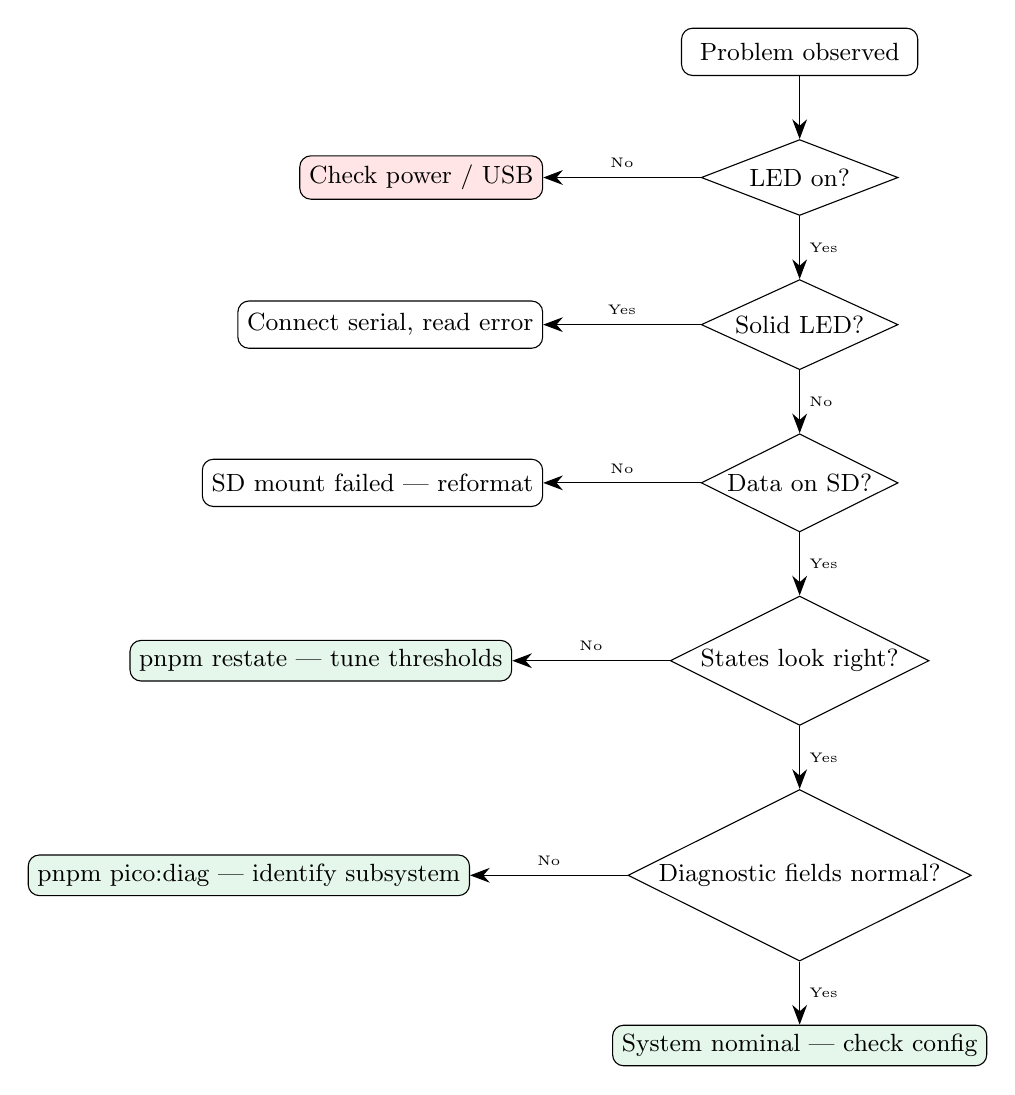
\begin{tikzpicture}[
    node distance=0.8cm,
    decision/.style={diamond, draw, aspect=2, minimum width=2.5cm, font=\small, inner sep=1pt},
    block/.style={draw, rounded corners, minimum width=3cm, minimum height=0.6cm, font=\small},
    result/.style={draw, rounded corners, minimum width=3cm, font=\small, fill=accentgreen!15},
    fail/.style={draw, rounded corners, minimum width=3cm, font=\small, fill=accentred!15},
    arr/.style={-{Stealth[length=2.5mm]}},
]
\node[block] (start) {Problem observed};
\node[decision, below=of start] (led) {LED on?};
\node[fail, left=2cm of led] (nopower) {Check power / USB};
\node[decision, below=of led] (solid) {Solid LED?};
\node[block, left=2cm of solid] (serial) {Connect serial, read error};
\node[decision, below=of solid] (logging) {Data on SD?};
\node[block, left=2cm of logging] (mount) {SD mount failed --- reformat};
\node[decision, below=of logging] (states) {States look right?};
\node[result, left=2cm of states] (restate) {pnpm restate --- tune thresholds};
\node[decision, below=of states] (diag) {Diagnostic fields normal?};
\node[result, left=2cm of diag] (bench) {pnpm pico:diag --- identify subsystem};
\node[result, below=of diag] (ok) {System nominal --- check config};

\draw[arr] (start) -- (led);
\draw[arr] (led) -- node[above, font=\tiny] {No} (nopower);
\draw[arr] (led) -- node[right, font=\tiny] {Yes} (solid);
\draw[arr] (solid) -- node[above, font=\tiny] {Yes} (serial);
\draw[arr] (solid) -- node[right, font=\tiny] {No} (logging);
\draw[arr] (logging) -- node[above, font=\tiny] {No} (mount);
\draw[arr] (logging) -- node[right, font=\tiny] {Yes} (states);
\draw[arr] (states) -- node[above, font=\tiny] {No} (restate);
\draw[arr] (states) -- node[right, font=\tiny] {Yes} (diag);
\draw[arr] (diag) -- node[above, font=\tiny] {No} (bench);
\draw[arr] (diag) -- node[right, font=\tiny] {Yes} (ok);
\end{tikzpicture}
\caption{Quick diagnostic flowchart. Start here when something goes wrong.}
\label{fig:diag-flow}
\end{figure}

% ══════════════════════════════════════════════════════
\section{Operational Procedures}
\label{sec:procedures}
% ══════════════════════════════════════════════════════

\subsection{First Boot (New Board)}
\begin{enumerate}
    \item Flash MicroPython v1.22+ onto Pico
    \item Copy \file{hw\_check.py} as \file{main.py}, reboot, check serial --- fix any FAILs
    \item Copy all avionics source folders to Pico root
    \item Copy \file{main.py} (flight firmware) to Pico root
    \item Ensure \file{sdcard.py} driver is present
    \item Boot --- preflight runs automatically
\end{enumerate}

\subsection{Pre-Flight (Pad)}
\begin{enumerate}
    \item Run \texttt{pnpm preflight} from laptop
    \item Verify GO on all checks
    \item Monitor live telemetry for stable altitude/velocity
    \item Disconnect USB --- board enters PAD state (slow blink)
\end{enumerate}

\subsection{Post-Flight}
\begin{enumerate}
    \item Run \texttt{pnpm postflight} or mount SD at \texttt{/Volumes/AVIONICS/}
    \item Decode: \texttt{pnpm decode /Volumes/AVIONICS/flight\_001/flight.bin}
    \item Review state transitions and diagnostic channels
    \item If states look wrong: \texttt{pnpm restate flight.bin -{}-plot}
    \item Compare with simulation: \texttt{pnpm simulator}
\end{enumerate}

\subsection{Changing Sample Rate}
Edit \config{SAMPLE\_RATE\_HZ} in \file{config.py}. Also adjust \config{LOG\_FLUSH\_EVERY} to maintain $\sim$\SI{1}{\second} flush intervals (e.g., 25\,Hz $\to$ \texttt{LOG\_FLUSH\_EVERY = 25}). Run timing test in \file{hw\_check.py} to verify headroom at new rate.

\subsection{Tuning the Kalman Filter}
\begin{itemize}
    \item Smoother output: decrease \config{KALMAN\_Q\_ALT} and \config{KALMAN\_Q\_VEL}
    \item Faster response: increase Q values
    \item Trust barometer more: decrease \config{KALMAN\_R\_ALT}
    \item Test by running \file{ground\_test.py} and comparing raw vs.\ filtered
    \item Validate with float precision diagnostic \xref{sec:diagnostics}
\end{itemize}

% ══════════════════════════════════════════════════════
\section{Known Limitations and Pitfalls}
\label{sec:known-issues}
% ══════════════════════════════════════════════════════

Hard-won lessons from v1.13.0 through v1.16.0 development. These are the things that will waste hours if you don't know about them.

\subsection{RP2040 / MicroPython Runtime}

\begin{table}[ht]
\centering
\small
\caption{Platform pitfalls. All discovered during flight firmware development.}
\label{tab:pitfalls}
\begin{tabularx}{\textwidth}{l X}
\toprule
\textbf{Pitfall} & \textbf{Details} \\
\midrule
USB CDC \texttt{print()} blocks & When no host reads the serial port, \texttt{print()} blocks indefinitely. \texttt{select.poll()} does \textit{not} reliably detect USB backpressure on RP2040. The firmware times the first in-loop print: if $>$\SI{50}{\milli\second}, all console output is permanently disabled for that session. \xref{sec:flight-loop} \\
\midrule
\texttt{gc.mem\_free()} is slow & Walks the entire heap bitmap. Costs \SI{1}{\milli\second}--\SI{3}{\milli\second}. Never call at \SI{50}{\hertz}. The firmware calls it once per second, preceded by \texttt{gc.collect()}. \\
\midrule
Python scoping trap & \texttt{\_flag = False} inside a function creates a \textit{local} variable. You must write \texttt{global \_flag} to modify the module-level variable. This caused the console auto-disable to silently fail for two firmware revisions. \\
\midrule
Hardware I\textsuperscript{2}C EIO bug & RP2040 native \texttt{I2C} raises \texttt{EIO} on this board. \textbf{Workaround:} SoftI2C (bit-banged) at \SI{100}{\kilo\hertz}. Slightly slower but reliable. \\
\midrule
Scratch register safety & SCRATCH0 and SCRATCH4 are used by MicroPython/bootrom. \textbf{Only SCRATCH6 and SCRATCH7 are safe.} Using SCRATCH0--4 will corrupt the boot sequence. \\
\midrule
\texttt{reset\_cause()} unreliable & WDT resets may report as PWRON\_RESET (value 1) if a brown-out triggers simultaneously. Don't rely solely on \texttt{reset\_cause() == 3}; also check the scratch register magic (\hex{DEAD}). \\
\midrule
\texttt{import} inside loops & \texttt{import time} inside \texttt{write\_frame()} is measurably slow in MicroPython. All imports must be at module level. \\
\bottomrule
\end{tabularx}
\end{table}

\subsection{9\,V Battery and Brown-Out}
\label{sec:battery}

The board runs on a 9\,V alkaline battery through buck/boost converters.

\begin{table}[ht]
\centering
\caption{9\,V alkaline battery state. Check \texttt{v\_9v\_mv} in \file{preflight.txt} before debugging software.}
\label{tab:battery}
\begin{tabular}{l l l}
\toprule
\textbf{Voltage} & \textbf{State} & \textbf{Action} \\
\midrule
9.4--9.6\,V & Fresh & Good to fly \\
8.0--9.0\,V & Good & Nominal \\
7.0--8.0\,V & Low & Replace before flight \\
$<$6.5\,V & Dead & \danger{Will cause brown-out crashes} \\
\bottomrule
\end{tabular}
\end{table}

\danger{Critical pattern:} At $\sim$\SI{6.2}{\volt}, the SD card flush current spike drops the 3.3\,V rail below the RP2040 brown-out threshold. This causes a PWRON reset (not a WDT reset) that looks like a power cycle, not a crash. The diagnostic signature is: frame count at an exact multiple of \config{LOG\_FLUSH\_EVERY} (50) in the crash report --- this means the crash happened at a flush boundary.

\textbf{Rule:} If the 9\,V rail reads below \SI{7}{\volt} in preflight, replace the battery before investigating any software issue.

\subsection{SD Card Considerations}
\label{sec:sd-notes}

\begin{itemize}
    \item \textbf{Format:} FAT32 only (MicroPython \texttt{os.VfsFat}). Cards must be pre-formatted before first use.
    \item \textbf{Speed class:} Use Class 10 / U1 or better. Cheap cards have unpredictable flush latency.
    \item \textbf{No hot-swap:} Card must be inserted before power-on. Inserting mid-flight will not be detected.
    \item \textbf{Initialisation:} SPI starts at \SI{400}{\kilo\hertz} (SD spec), 80 dummy clocks with CS high, then ramps to \SI{10}{\mega\hertz}.
    \item \textbf{\texttt{os.sync()} availability:} Some MicroPython builds lack it. The firmware prints a warning and continues without FAT metadata sync --- data is at higher risk on power loss.
    \item \textbf{Driver:} Uses the standard MicroPython \texttt{sdcard.py} from \texttt{micropython-lib}. Must be present on the Pico filesystem.
\end{itemize}

\subsection{Barometer Limitations}

\begin{itemize}
    \item \textbf{Altitude ceiling:} Hypsometric formula (Eq.~\ref{eq:altitude}) is valid in the troposphere (0--\SI{11000}{\metre}). Above this, the lapse rate changes.
    \item \textbf{No accelerometer:} Velocity is inferred from pressure alone. High-frequency vibration and spin are invisible to the filter.
    \item \textbf{Wind sensitivity:} Dynamic pressure from airflow over the barometer port biases the reading. Mount the sensor in a still-air cavity.
    \item \textbf{Calibration sanity:} If AC1 = 0 or AC1 = $-$1, the EEPROM is blank or corrupted. The driver raises \texttt{RuntimeError}.
    \item \textbf{Cold-start garbage:} The BMP180 occasionally returns an out-of-range reading on the first conversion after power-on. The 20-sample Kalman priming sequence absorbs this.
\end{itemize}

% ══════════════════════════════════════════════════════
\section{Software Dependencies}
\label{sec:dependencies}
% ══════════════════════════════════════════════════════

\subsection{On-Device (Pico)}

\begin{table}[ht]
\centering
\caption{Pico firmware dependencies.}
\label{tab:pico-deps}
\begin{tabularx}{\textwidth}{l l X}
\toprule
\textbf{Dependency} & \textbf{Version} & \textbf{Notes} \\
\midrule
MicroPython & $\geq$ 1.22 & Official RP2040 build. Requires Timer(-1), SoftI2C, mem32, WDT, reset\_cause \\
\texttt{sdcard.py} & --- & From \texttt{micropython-lib}. Must be copied to Pico filesystem \\
\bottomrule
\end{tabularx}
\end{table}

Built-in modules used: \texttt{machine} (Pin, SPI, SoftI2C, ADC, Timer, WDT, freq, reset\_cause, mem32), \texttt{time}, \texttt{os}, \texttt{gc}, \texttt{struct}, \texttt{sys}.

\subsection{Laptop (Ground Station)}

\begin{table}[ht]
\centering
\caption{Laptop-side dependencies for ground station tools.}
\label{tab:laptop-deps}
\begin{tabularx}{\textwidth}{l l X}
\toprule
\textbf{Dependency} & \textbf{Required by} & \textbf{Install} \\
\midrule
Python 3.9+ & All tools & System package manager \\
\texttt{rich} & preflight, postflight, pico\_diag, restate TUIs & \texttt{pip3 install rich} \\
\texttt{pyserial} & preflight, postflight, pico\_diag (USB serial) & \texttt{pip3 install pyserial} \\
\texttt{matplotlib} & decode\_log (optional plots) & \texttt{pip3 install matplotlib} \\
\texttt{numpy} & simulate, decode\_log (optional) & \texttt{pip3 install numpy} \\
\texttt{pytest} & test suite & \texttt{pip3 install pytest} \\
Node.js + pnpm & Script runner, ground station web UI & \texttt{brew install node pnpm} \\
\bottomrule
\end{tabularx}
\end{table}

\texttt{matplotlib} and \texttt{numpy} are optional --- tools that use them provide helpful error messages if missing.

% ══════════════════════════════════════════════════════
\section{Serial Output Reference}
\label{sec:serial-output}
% ══════════════════════════════════════════════════════

Connect to the Pico via USB serial at \textbf{115200 baud}. The firmware prints status during boot and once per second during the flight loop.

\subsection{Normal Boot}

\begin{lstlisting}[basicstyle=\ttfamily\scriptsize]
+==========================================+
|   UNSW ROCKETRY - MPR ALTITUDE LOGGER    |
+==========================================+

LED GUIDE:
  Fast blink (250ms) = booting / preflight running
  Solid ON           = ERROR (check serial)
  Slow blink (1s)    = PAD - ready, safe to disconnect USB
  Triple flash       = LANDED - data saved

[1/7] Overclock        200 MHz
[2/7] LED started      fast blink = preflight running
[3/7] SD card ...      OK - 7452.3 MB free -> /sd/flight_001/flight.bin
[4/7] Barometer ...    OK - 101325 Pa, 23.5C
[5/7] Power rails ...  OK - 3V3=3312 mV 5V=5023 mV 9V=9145 mV
[6/7] Calibrating ...  OK - ground P=101325 Pa
[7/7] Logger open      /sd/flight_001/flight.bin

+==========================================+
|  ALL PREFLIGHT CHECKS PASSED             |
|  LED: slow blink = PAD (waiting)         |
|  Logging at 50 Hz                        |
+==========================================+

[RDY] Waiting for launch...
[PAD    ] alt=  0.0m  vel= +0.0m/s  P=101325Pa  T=23.5C  3V3=3312mV  50Hz 2150us  #50
\end{lstlisting}

\subsection{Crash Reboot (WDT Reset)}

\begin{lstlisting}[basicstyle=\ttfamily\scriptsize]
[CRASH REBOOT] Previous session ended in WDT reset
  Last frame: #12450  t=249000 ms  RAM=48200 B  flush=3200 us
  Fast-rebooting to resume logging...

[FAST] SD=OK Baro=OK
[FAST] Logger: /sd/flight_002/flight.bin
[FAST] Logging at 50 Hz - crash reboot complete
\end{lstlisting}

\subsection{Preflight Failure (SD Card)}

\begin{lstlisting}[basicstyle=\ttfamily\scriptsize]
[1/7] Overclock        200 MHz
[2/7] LED started      fast blink = preflight running
[3/7] SD card ...      FAIL - mount failed (3 attempts)

+==========================================+
|  PREFLIGHT FAILED - LED IS SOLID ON      |
|  - SD card mount failed                  |
|  Ctrl-C to abort, or wait 10s            |
+==========================================+
  10... 9... 8... (countdown)

[FATAL] Cannot log without SD card. LED will stay solid.
\end{lstlisting}

\subsection{In-Flight Console Output (1\,Hz)}

\begin{lstlisting}[basicstyle=\ttfamily\scriptsize]
[PAD    ] alt=  0.1m  vel= +0.0m/s  P=101320Pa  T=23.5C  3V3=3310mV  50Hz 2140us  #500
[BOOST  ] alt= 42.3m  vel=+78.2m/s  P=100840Pa  T=23.1C  3V3=3305mV  50Hz 2200us  #550
[COAST  ] alt=285.6m  vel=+32.1m/s  P= 97960Pa  T=21.8C  3V3=3308mV  50Hz 2160us  #600
\end{lstlisting}

Console output is automatically disabled if USB is disconnected (print blocks $>$\SI{50}{\milli\second}). This is permanent for the session --- reconnecting USB will not re-enable it.

% ══════════════════════════════════════════════════════
\appendix
\section{Crash Report Format}
\label{sec:crash-report-format}

Written to \file{/sd/flight\_NNN/crash.txt} when the firmware detects a previous WDT reset:

\begin{lstlisting}[basicstyle=\ttfamily\scriptsize]
CRASH REPORT - Previous session ended in WDT reset
==================================================
Reboot reason: 3 (WDT_RESET)
Last frame: #12450
Last timestamp: 249000 ms
Free RAM: 48200 bytes (47 KB)
Last flush: 3200 us
State: COAST (2)
Flags: 0x00
CPU temp: 35 C
\end{lstlisting}

\textbf{Key diagnostic signals:}
\begin{itemize}
    \item Frame count at exact multiple of 50 $\to$ crash during flush \xref{sec:battery}
    \item State = BOOST or COAST $\to$ crash during active flight (vibration? power?)
    \item High CPU temp ($>$\SI{60}{\degreeCelsius}) $\to$ thermal issue
    \item Flags = 0x08 $\to$ SD card was already failing before crash
\end{itemize}

\section{Preflight Metadata Format}
\label{sec:preflight-format}

Written to \file{/sd/flight\_NNN/preflight.txt} at boot:

\begin{lstlisting}[basicstyle=\ttfamily\scriptsize]
UNSW Rocketry - MPR Altitude Logger
Avionics v1.16.0
MicroPython v1.22.0 on 2024-01-05; Raspberry Pi Pico with RP2040
Boot time: 3450 ms
Reboot reason: PWRON
Crash reboot: No
Manual override: No
Errors: (none)
Ground pressure: 101325 Pa
Voltages: 3V3=3312 mV  5V=5023 mV  9V=9145 mV
Warnings: (none)
Barometer: OK
Sample rate: 50 Hz
Log file: /sd/flight_001/flight.bin
Log format: v3, 40 bytes/frame
\end{lstlisting}

\vspace{2em}
\hrule
\vspace{0.5em}
\begin{center}
\small\textit{MPR Altitude Logger v1.16.0 --- UNSW Rocketry --- AURC 2026}
\end{center}

\end{document}
